\documentclass{article} % For LaTeX2e
\usepackage{nips15submit_e,times}
\usepackage{hyperref}
\usepackage{url}
\usepackage{graphicx}
\usepackage{amsfonts}
\usepackage{amsmath}
\usepackage{caption}
\usepackage{subcaption}
%\documentstyle[nips14submit_09,times,art10]{article} % For LaTeX 2.09


\title{Handwritten Digits Classification using Logistic and Softmax Regression}


\author{
Sriram Ravindran\\
Department of Computer Science\\
A53208651 \\
\texttt{sriram@ucsd.edu} \\
\And
Ojas Gupta \\
A53201624 \\
\texttt{ogupta@ucsd.edu} \\
}

% The \author macro works with any number of authors. There are two commands
% used to separate the names and addresses of multiple authors: \And and \AND.
%
% Using \And between authors leaves it to \LaTeX{} to determine where to break
% the lines. Using \AND forces a linebreak at that point. So, if \LaTeX{}
% puts 3 of 4 authors names on the first line, and the last on the second
% line, try using \AND instead of \And before the third author name.

\newcommand{\fix}{\marginpar{FIX}}
\newcommand{\new}{\marginpar{NEW}}

%\nipsfinalcopy % Uncomment for camera-ready version

\begin{document}


\maketitle
\begin{abstract}
Here in this project we have implemented the famous Logistic Regression which is a two class classifier and its extension Softmax Regression which is a multiclass classifier. Both of these methods are trained and tested on famous handwritten MNIST dataset via gradient descent. We used the first 20000 data points as our training set out of which we have kept the 10 percent i.e. 2000 as our hold out set. On training our system we have tested on the first 2000 test data points so as to evaluate our work. On using the Logistic Regression, we have attained an accuracy of " " while classifying 2 vs 3 and an accuracy " " while classifying 2 vs 8. On applying 10 way classification, we get an accuracy of " ". To enhance classification and generalization we have used regularization as well. 
\end{abstract}

\section{Derivation of Gradient for Logistic Regression}
We will derive the gradient for logistic regression by using the following predefined variables given in the document.

Given:
\begin{center}
	$y^n=\cfrac{1}{1+exp(-w^T x^n)}$(Sigmoid function)\\
    \hfill\break
    $E(w) = -\sum_N t^n lny^n + (1-t^n) ln(1-y^n)$\\
    \hfill\break
\end{center}
To Prove:
\begin{center}
    -$\cfrac{\partial E^n(w)}{\partial w_j} = (t^n-y^n)x^n_j $\\
    \hfill\break
\end{center}
\begin{center}
Let's recall the properties of Sigmoid Function, if $\sigma(x)$ is a sigmoid function then following two properties hold:\\
\hfill\break
1) $\sigma(x)=1-\sigma(-x)$\\
\hfill\break
2) $\sigma'(x)=\sigma(x)\sigma(-x)$\\
\hfill\break
\end{center}
Derivation:
\begin{center}
$E^n(w) = -(t^n lny^n + (1-t^n) ln(1-y^n))$\\
\hfill\break
\hfill\break
$\cfrac{\partial E^n(w)}{\partial w_j} = -(\cfrac{t^n}{y^n} - \cfrac{1-t^n}{1-y^n})\cfrac{\partial y^n}{\partial w_j}$\\
    \hfill\break
    \hfill\break
$\cfrac{\partial E^n(w)}{\partial w_j} = -(\cfrac{t^n-y^n}{y^n(1-y^n)})\cfrac{\partial y^n}{\partial w_j}$\\
    \hfill\break
    \hfill\break
$\cfrac{\partial E^n(w)}{\partial w_j} = -(\cfrac{t^n-y^n}{y^n(1-y^n)})y^n(1-y^n)\cfrac{\partial w^Tx}{\partial w_j}$(Properties of Sigmoid)\\
    \hfill\break
    \hfill\break
$\cfrac{\partial E^n(w)}{\partial w_j} = -(t^n-y^n)\cfrac{\partial w^Tx^n}{\partial w_j}$\\
    \hfill\break
    \hfill\break
$\cfrac{\partial E^n(w)}{\partial w_j} = -(t^n-y^n)x^n_j$\\
    \hfill\break
    Hence Proved 

\end{center}
\section{Derivation of Gradient for Softmax Regression}
We will derive the gradient for softmax regression by using the following predefined variables given in the document.

Given:
\begin{center}
	$y_k^n = \cfrac{exp(a_{k}^n)}{\sum_k' exp(a_k'^n)}$\\
    \hfill\break
$a_{k}^n = w_k^T x^n$\\
\hfill\break
$E = −\sum_n \sum_{k=1}^{c} t^n_k ln(y_k^n)$
\end{center}
To Prove:
\begin{center}
    -$\cfrac{\partial E^n(w)}{\partial w_j^k} = (t^n_k-y^n_k)x^n_j $\\
    \hfill\break
\end{center}
Derivation:
\begin{center}
$E^n(w) = -\sum_{k'=1}^{c} t^n_{k'} ln(y_{k'}^n)$\\
\hfill\break
\hfill\break
$\cfrac{\partial E^n(w)}{\partial w_{jk}} = -\sum_{k'=1}^{c}\cfrac{\partial(t^n_{k'}ln(exp(w_{k'}^Tx^n))-t^n_{k'}ln(\sum_{k''}exp(w_{k''}^Tx^n)))}{\partial w_{jk}}$\\
	\hfill\break
    \hfill\break
$\cfrac{\partial E^n(w)}{\partial w_{jk}} = -\sum_{k'=1}^{c}\cfrac{\partial(t^n_{k'}w_{k'}^Tx^n-t^n_{k'}ln(\sum_{k''}exp(w_{k''}^Tx^n)))}{\partial w_{jk}}$\\
    \hfill\break
    \hfill\break
$\cfrac{\partial E^n(w)}{\partial w_{jk}} = -t^n_kx^n_j-\sum_{k'=1}^{c}\cfrac{\partial (t^n_{k'}ln(\sum_{k''}exp(w_{k''}^Tx^n)))}{\partial w_{jk}}$\\
    \hfill\break
    \hfill\break
$\cfrac{\partial E^n(w)}{\partial w_{jk}} = -t^n_kx^n_j-\cfrac{\partial (ln(\sum_{k''}exp(w_{k''}^Tx^n)))}{\partial w_{jk}}$\\
    \hfill\break
    \hfill\break
$\cfrac{\partial E^n(w)}{\partial w_{jk}} = -t^n_kx^n_j-\cfrac{exp(w_k^Tx^n)}{\sum_{k''}exp(w_{k''}^Tx^n))}x^n_j$\\
    \hfill\break
    \hfill\break
$\cfrac{\partial E^n(w)}{\partial w_{jk}} = -t^n_kx^n_j-y_k^nx^n_j$\\
    \hfill\break
    \hfill\break
$\cfrac{\partial E^n(w)}{\partial w_{jk}} = -(t^n_k-y_k^n)x^n_j$\\
    \hfill\break
    Hence Proved 

\end{center}

\section{Logistic Regression}
Logistic regression can be modeled as using a single neuron reading in an input vector (1,{\sl x}) $\in \mathbb{R}^{d+1}$ and parameterized by weight vector {\sl w} $\in \mathbb{R}^{d+1}$ . d is the dimensionality of the input, and we tack on a "1" at the beginning for a bias parameter, $w_0$ . The neuron outputs the probability that x is a member of class $C_1$.\\
\begin{center}
P $(x \in C_1 |x) = \cfrac{1}{1+exp(-w^T x)}$\\
\hfill\break
\hfill\break
P $(x \in C_2 |x)$ = 1 − P$(x \in C_1 |x)$\\
\hfill\break
\end{center}

Cross entropy loss function for two categories over the training examples is given as following.\\

\begin{center}
$E^n(w) = -(t^n lny^n + (1-t^n) ln(1-y^n))$\\
\hfill\break
\hfill\break
\end{center}

Here, $t^n$ is the target or teaching signal for example n. Our goal is to optimize this cost function via gradient descent. This cost function is minimized at 0 when $t^n = y^n$ for all n.
\subsection{Introduction}
Using the gradient derived for Logistic Regression cross entropy loss, we will first use gradient descent to classify for categories: 2's and 3's, 2's and 8's.  

We have taken the data from the famous MNIST handwritten data, of which we used the first 20000 as our training data set, and 2000 from the testing data set. Out of the training data set we have excluded 2000 data points for the hold out set.\\
\subsection{Method}
\subsection{Results and Discussion}

We have calculated the entropy and classification accuracy of 2 vs 3 and 2 vs 8 data set and the results are found to be quite impressive. Following are the graphs plotted for them. Figure 1 and 2 shows the entropy and classification accuracy of 2 vs 3

\begin{figure}[h]
\begin{center}
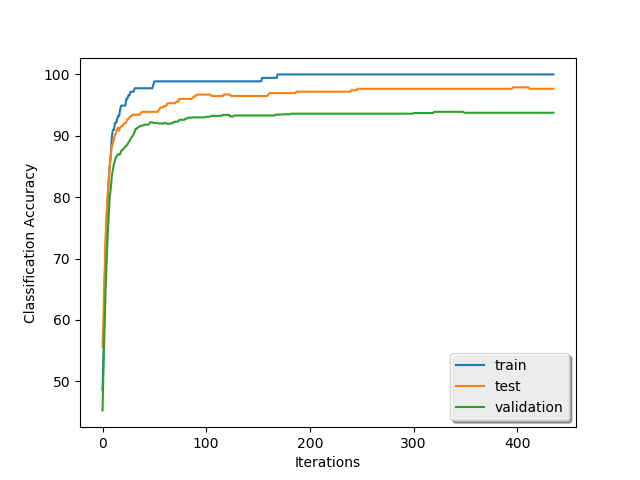
\includegraphics[width=0.8\linewidth]{plt_2vs3_accuracy.png}
\end{center}
\caption{Plot of accuracy in 2 vs 3.}
\end{figure}

\begin{figure}[h]
\begin{center}
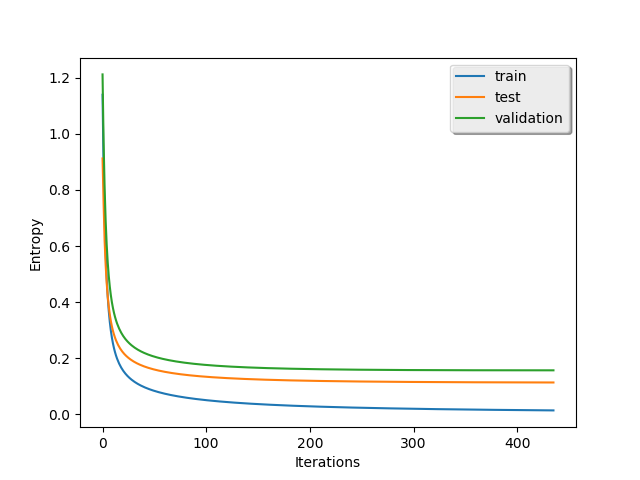
\includegraphics[width=0.8\linewidth]{plt_2vs3_losses.png}
\end{center}
\caption{Plot of entropy in 2 vs 3.}
\end{figure}

\begin{figure}[h]
\begin{center}
%\framebox[4.0in]{$\;$}
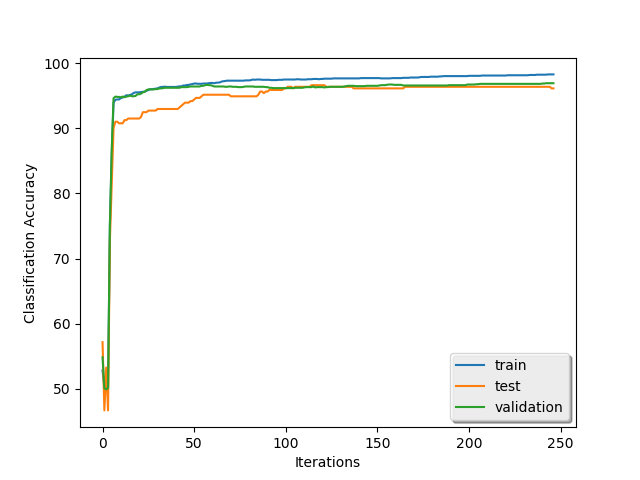
\includegraphics[width=0.8\linewidth]{plt_2vs8_accuracy.png}
\end{center}
\caption{Plot of accuracy in 2 vs 8.}
\end{figure}

\begin{figure}[h]
\begin{center}
%\framebox[4.0in]{$\;$}
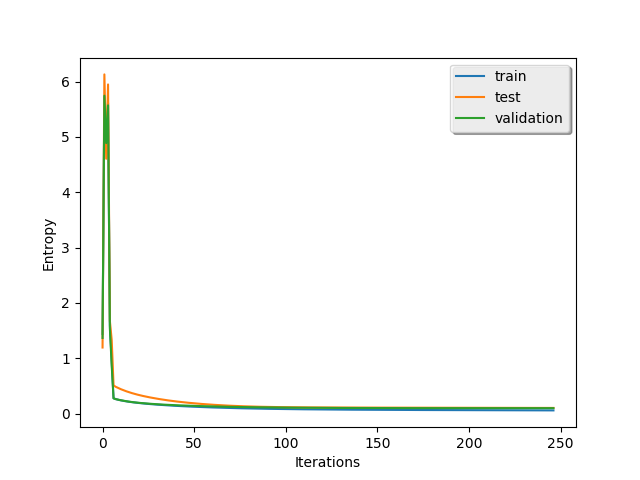
\includegraphics[width=0.8\linewidth]{plt_2vs8_losses.png}
\end{center}
\caption{Plot of losses in 2 vs 8.}
\end{figure}
As the "hold-out" set is previously unseen, it acts as a good replacement for the testing data, as can be seen from the results.
\begin{figure}[h]
\begin{center}
%\framebox[4.0in]{$\;$}
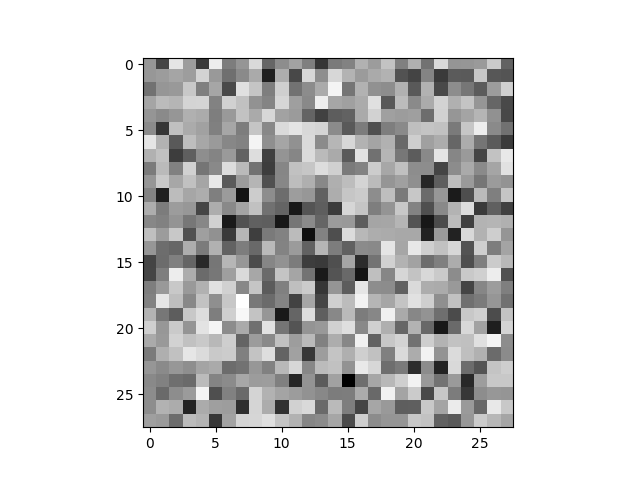
\includegraphics[width=0.8\linewidth]{2vs3-2vs8.png}
\end{center}
\caption{Subtraction of 2 vs 3 Classifier and 2 vs 8 Classifier.}
\end{figure}

\begin{figure}[h]
\begin{center}
%\framebox[4.0in]{$\;$}
\includegraphics[width=0.8\linewidth]{2vs3.png}
\end{center}
\caption{2vs3.}
\end{figure}

\begin{figure}[h]
\begin{center}
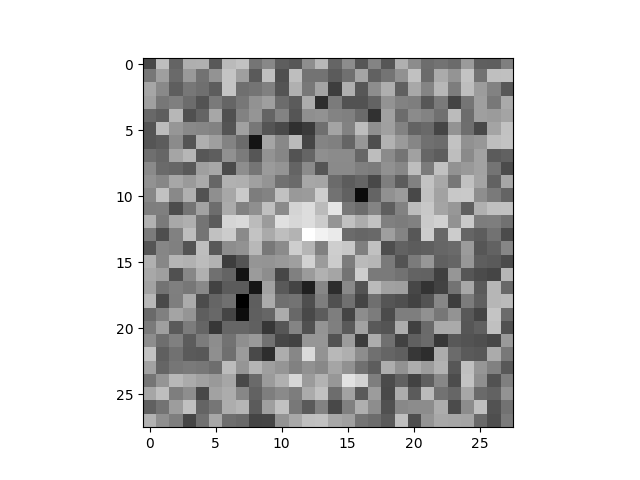
\includegraphics[width=0.8\linewidth]{2vs8.png}
\end{center}
\caption{2 vs 8 Classifier weights as an image.}
\end{figure}
d) While a pattern is not clear from the image, the darker a cell in the image, the more those cells contribution towards two-ness in the image. The difference image must contain features (dark cells) which are neither in three nor in eight.
\section{Regularization}

Part b:
\begin{figure}[h]
\begin{center}
\includegraphics[width=0.8\linewidth]{Reg_L1/2vs3.png}
\end{center}
\caption{Training Accuracy with L1 regularization with different lambda.}
\end{figure}

\begin{figure}[h]
\begin{center}
\includegraphics[width=0.8\linewidth]{Red_L2/2vs3.png}
\end{center}
\caption{Training Accuracy on L2.}
\end{figure}

Part c:
\begin{figure}[h]
\begin{center}
\includegraphics[width=0.8\linewidth]{Reg_L1/2vs3w_len.png}
\end{center}
\caption{Length of weight vector on L1.}
\end{figure}

\begin{figure}[h]
\begin{center}
\includegraphics[width=0.8\linewidth]{Red_L2/2vs3w_len.png}
\end{center}
\caption{Length of weight vector on L2.}
\end{figure}

Part d:

\begin{figure}
\centering
\begin{subfigure}{.6\textwidth}
	\centering
	\includegraphics[width=0.7\linewidth]{Reg_L1/test.png}
	\caption{Testing error vs log$\lambda$ on L1.}
\end{subfigure}%
\begin{subfigure}{.6\textwidth}
    \centering
	\includegraphics[width=0.7\linewidth]{Red_L2/test.png}
	\caption{Testing error vs log$\lambda$ on L2.}
\end{subfigure}
\end{figure}

Part e:

$lambda$=0.01

\begin{figure}[h]
\begin{center}
\includegraphics[width=0.8\linewidth]{Reg_L1/0_01.png}
\end{center}
\caption{Testing error vs log$\lambda$ on L1.}
\end{figure}

\begin{figure}[h]
\begin{center}
\includegraphics[width=0.8\linewidth]{Red_L2/2vs30_01.png}
\end{center}
\caption{Testing error vs log$\lambda$ on L2.}
\end{figure}

$lambda$=0.001

\begin{figure}[h]
\begin{center}
\includegraphics[width=0.8\linewidth]{Reg_L1/0_001.png}
\end{center}
\caption{Testing error vs log$\lambda$ on L1.}
\end{figure}

\begin{figure}[h]
\begin{center}
\includegraphics[width=0.8\linewidth]{Red_L2/2vs30_001.png}
\end{center}
\caption{Testing error vs log$\lambda$ on L2.}
\end{figure}

$lambda$=0.0001

\begin{figure}[h]
\begin{center}
\includegraphics[width=0.8\linewidth]{Reg_L1/0_0001.png}
\end{center}
\caption{Testing error vs log$\lambda$ on L1.}
\end{figure}

\begin{figure}[h]
\begin{center}
\includegraphics[width=0.8\linewidth]{Red_L2/2vs30_0001.png}
\end{center}
\caption{Testing error vs log$\lambda$ on L2.}
\end{figure}

$lambda$=0.00001

\begin{figure}[h]
\begin{center}
\includegraphics[width=0.8\linewidth]{Reg_L1/0_00001.png}
\end{center}
\caption{Testing error vs log$\lambda$ on L1.}
\end{figure}

\begin{figure}[h]
\begin{center}
\includegraphics[width=0.8\linewidth]{Red_L2/2vs30_00001.png}
\end{center}
\caption{Testing error vs log$\lambda$ on L2.}
\end{figure}


\section{Softmax Regression}
Softmax regression is the generalization of logistic regression for multiple (c) classes. Now given an input $x^n$ , softmax regression will output a vector $y^n$ , where each element, $y_k^n$ represents the probability that $x^n$ is in class k.\\
\begin{center}
$y_k^n = \frac{exp(a_{k}^n)}{\sum_k' exp(a_k'^n)}$\\
$a_{k}^n = w_k^T x^n$\\
\end{center}

Here, $a_{k}^n$ is called the net input to output unit $y_k$. Note each output has its own weight vector $w_k$ . With our model defined, we now define the cross-entropy cost function for multiple categories:
\begin{center}
$E = −\sum_n \sum_{k=1}^{c} t^n_k ln(y_k^n)$
\end{center}

Again, taking the average of this over the number of training examples normalizes this error over different training set sizes.

Further information is distributed as section 3.1 contains the introduction to the problem, section 3.2 contains method used to solve the problem. Results ans Discussion is done in section 3.3 and 3.4 respectively.\\ 
\subsection{Introduction}
In this part of the problem, we have created a multiclass classifier which classifies a data point into 10 different classes. We have taken the data from the famous MNIST handwritten data, of which we used the first 20000 as our training data set, and 2000 from the testing data set. Out of the training data set we have excluded 2000 data points for the hold out set.\\
\subsection{Method}
\subsection{Results and Discussion}

Here, as instructed in the part(a) we have used a hold out set and Regularization in the softmax regression problem so as to classify handwritten data set in 10 classes.

Here the type of Regularization from which we received the maximum accuracy of hold out set was L2 and the value of $\lambda$ = 0.00001. Here We checked the method for other values of $\lambda$ as well mainly [0.1, 0.01, 0.001, 0.0001, 0.0000] with both L1 and L2 Regularization and found L2, 0.00001 to the most appropriate one.

As asked in the part 6(b), following is the graph of loss function with $\lambda$=0.00001.
\begin{figure}[h]
\begin{center}
\includegraphics[width=0.8\linewidth]{softmax/Entropy_vs_Iterations.png}
\end{center}
\caption{Part 6(c):Entropy vs Iterations of Softmax Regression with $\lambda$=0.00001.}
\end{figure}

As asked in the part 6(c), following is the graph of classification accuracy with $\lambda$=0.00001.

\begin{figure}[h]
\begin{center}
\includegraphics[width=0.8\linewidth]{softmax/Classification_Accuracy.png}
\end{center}
\caption{Part 6(b):Classification Accuracy of Softmax Regression with $\lambda$=0.00001.}
\end{figure}

\end{document}
